\chapter{Results}

\section{Workshop Study}
Descrition using max circ and shirt length

Finished garment eases per body area over 6 finished participants

Likert scales on per body area fit and comfort over all participants

Used vs Ideal efficiency metrics

\subsection{Distributions}
\subsubsection{Max Bodice Circ and Shirt Length}
Max bodice circumference and shirt length metrics are used to describe the initial dataset as they are the two most influential measurments on pattern width and pattern height, respectively.
Workshop study participants have a mean maximum bodice circumferemce of 99.96 cm, median of 98.50 cm and a standard deviation of 8.00 cm. The mean shirt length is 60.36 cm, median of 59.70 cm, and a standard deviation of 6.99 cm.
\begin{figure}[H]
    \centering
    \begin{subfigure}[b]{0.45\textwidth}
        \centering
        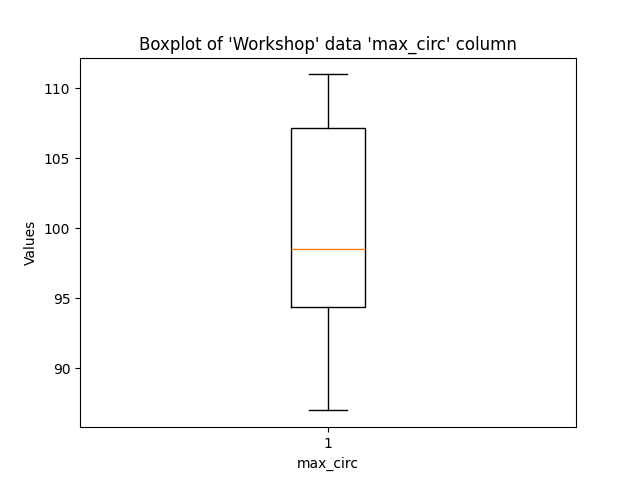
\includegraphics[width=\textwidth]{Images/Workshop_max_circ_Boxplot.png}
        \caption{}
    \end{subfigure}
    \hfill
    \begin{subfigure}[b]{0.45\textwidth}
        \centering
        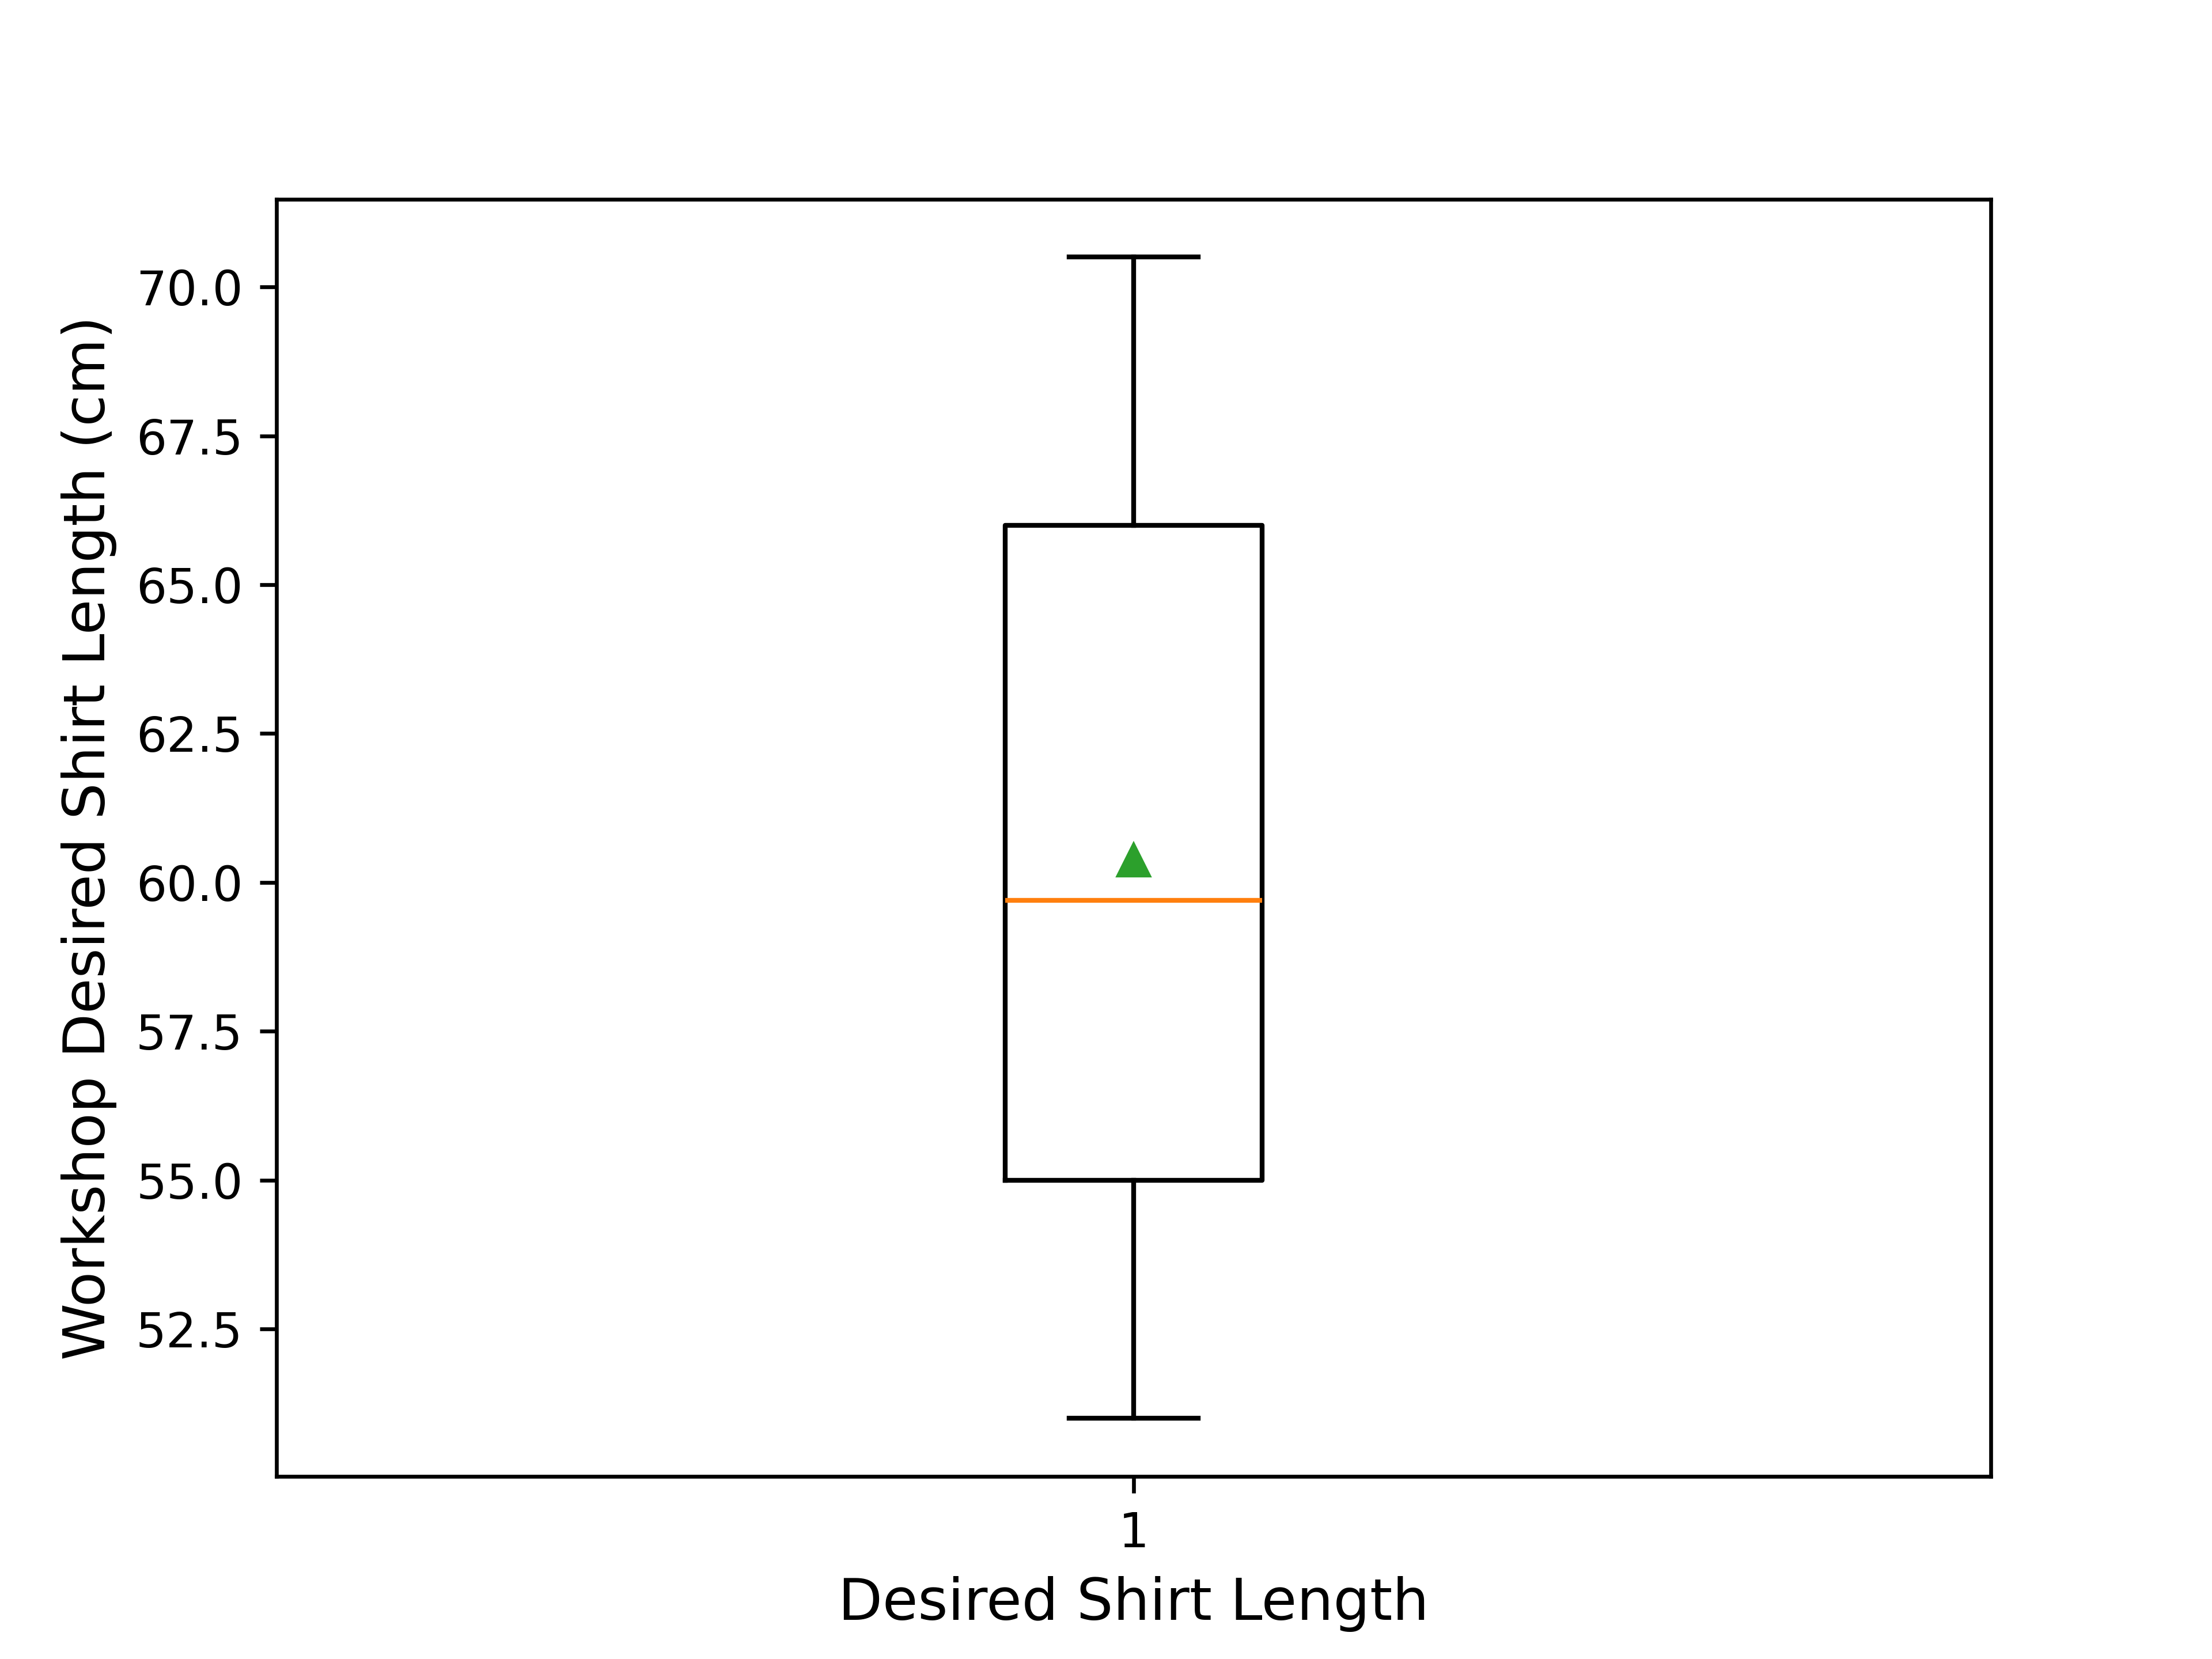
\includegraphics[width=\textwidth]{Images/Workshop_desired_shirt_length_Boxplot.png}
        \caption{}
    \end{subfigure}
    \caption{}
\end{figure}

\subsection{Learnings}
Beyond the metrics gathered, there were some additional insights gained from the workshop:
\subsubsection{Precisions}
All body measurements used in the workshop were rounded up to 0.5cm ceilings. While this does affect the fit (slightly looser) and efficiency (minimally higher) it does not affect the analysis that much. The reason for this is that this pattern is not machine cut. The target audience is confident beginners and not industrial tailors. Therefore, precise millimetre level cutting was not a fair expectation.

\subsubsection{Ease, Fit and Comfort}
\begin{figure} [H] % opens the figure environment. the '[H]' forces the image to be Here
    \centering % puts the image in the horizontal centre of the page
    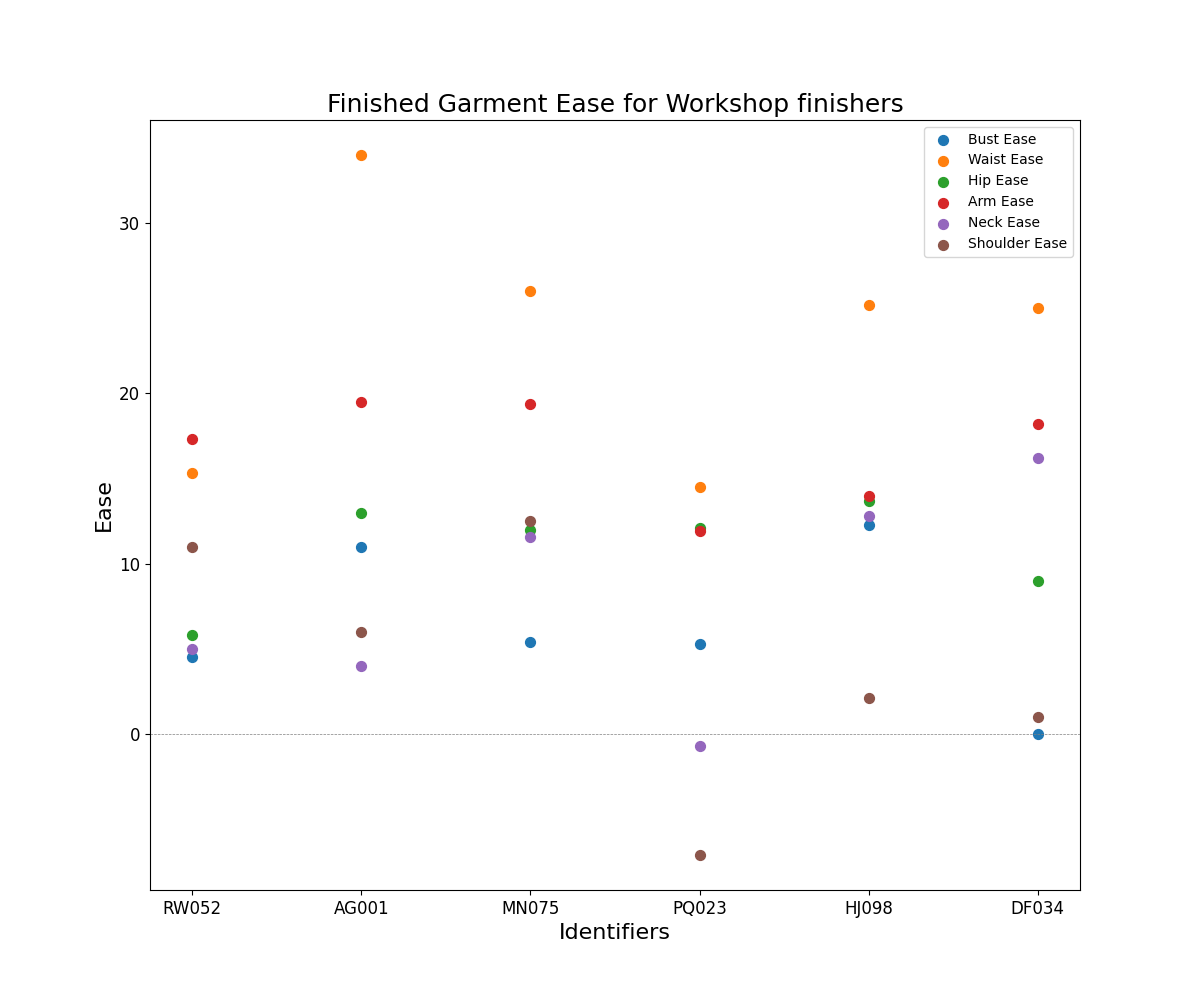
\includegraphics[width = 0.75\textwidth]{Images/FG_Ease_Plot.png} %this tells latex what graphics to include. I put my images in an 'Images' folder to aid file management, hence the Images/ before the file name. the width bit before allows you to alter the width of the image. It is also possible to use scale as well as using equations with the textwidth to make it say half the text width.
    \caption{Finished Garment eases for workshop participants}
\end{figure}

Add likert scale plots

\subsubsection{Fabric Use}
Efficiency, bolt width, cut loss width, and cut loss area for 100 scans study comparing ideal bolt and actual used bolt.
\begin{figure} [H] % opens the figure environment. the '[H]' forces the image to be Here
    \centering % puts the image in the horizontal centre of the page
    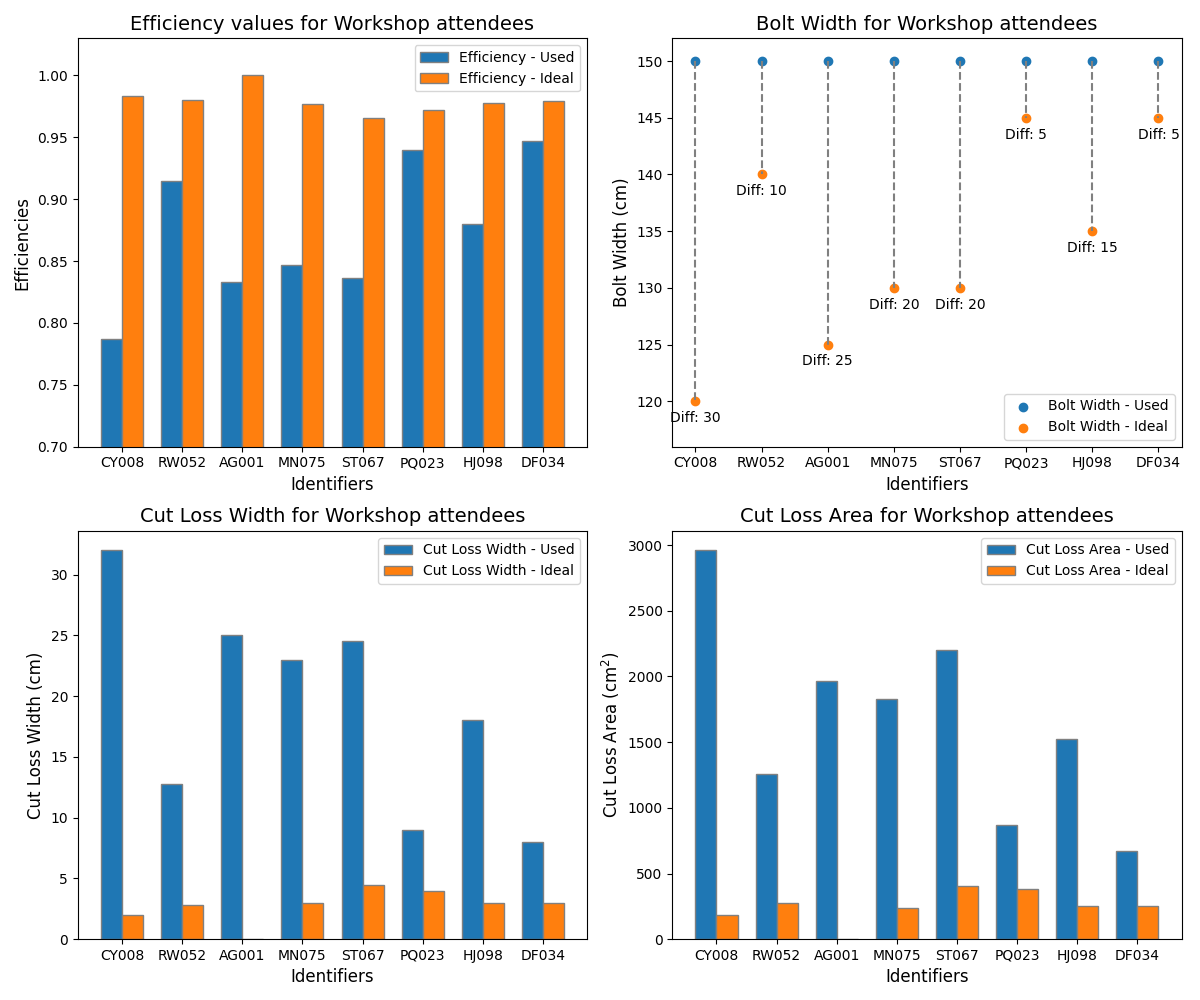
\includegraphics[width = 0.75\textwidth]{Images/Workshop_Plot.png} %this tells latex what graphics to include. I put my images in an 'Images' folder to aid file management, hence the Images/ before the file name. the width bit before allows you to alter the width of the image. It is also possible to use scale as well as using equations with the textwidth to make it say half the text width.
    \caption{Used and Ideal Efficiency Metrics for Workshop Study}
\end{figure}



\section{100 Body Scans Study findings}
\subsection{Distibutions}
100 Scans Study persons have a mean maximum bodice circumferemce of 99.58 cm, median of 98.25 cm and a standard deviation of 8.61 cm. The mean shirt length is  cm, median of  cm, and a standard deviation of  cm.

Need to add shirt length plots
\begin{figure}[H]
    \centering
    \begin{subfigure}[b]{0.45\textwidth}
        \centering
        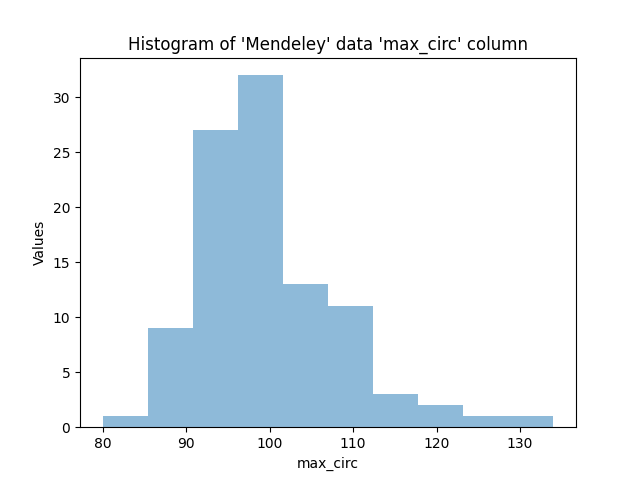
\includegraphics[width=\textwidth]{Images/Mendeley_max_circ_Hist.png}
        \caption{Histogram}
    \end{subfigure}
    \hfill
    \begin{subfigure}[b]{0.45\textwidth}
        \centering
        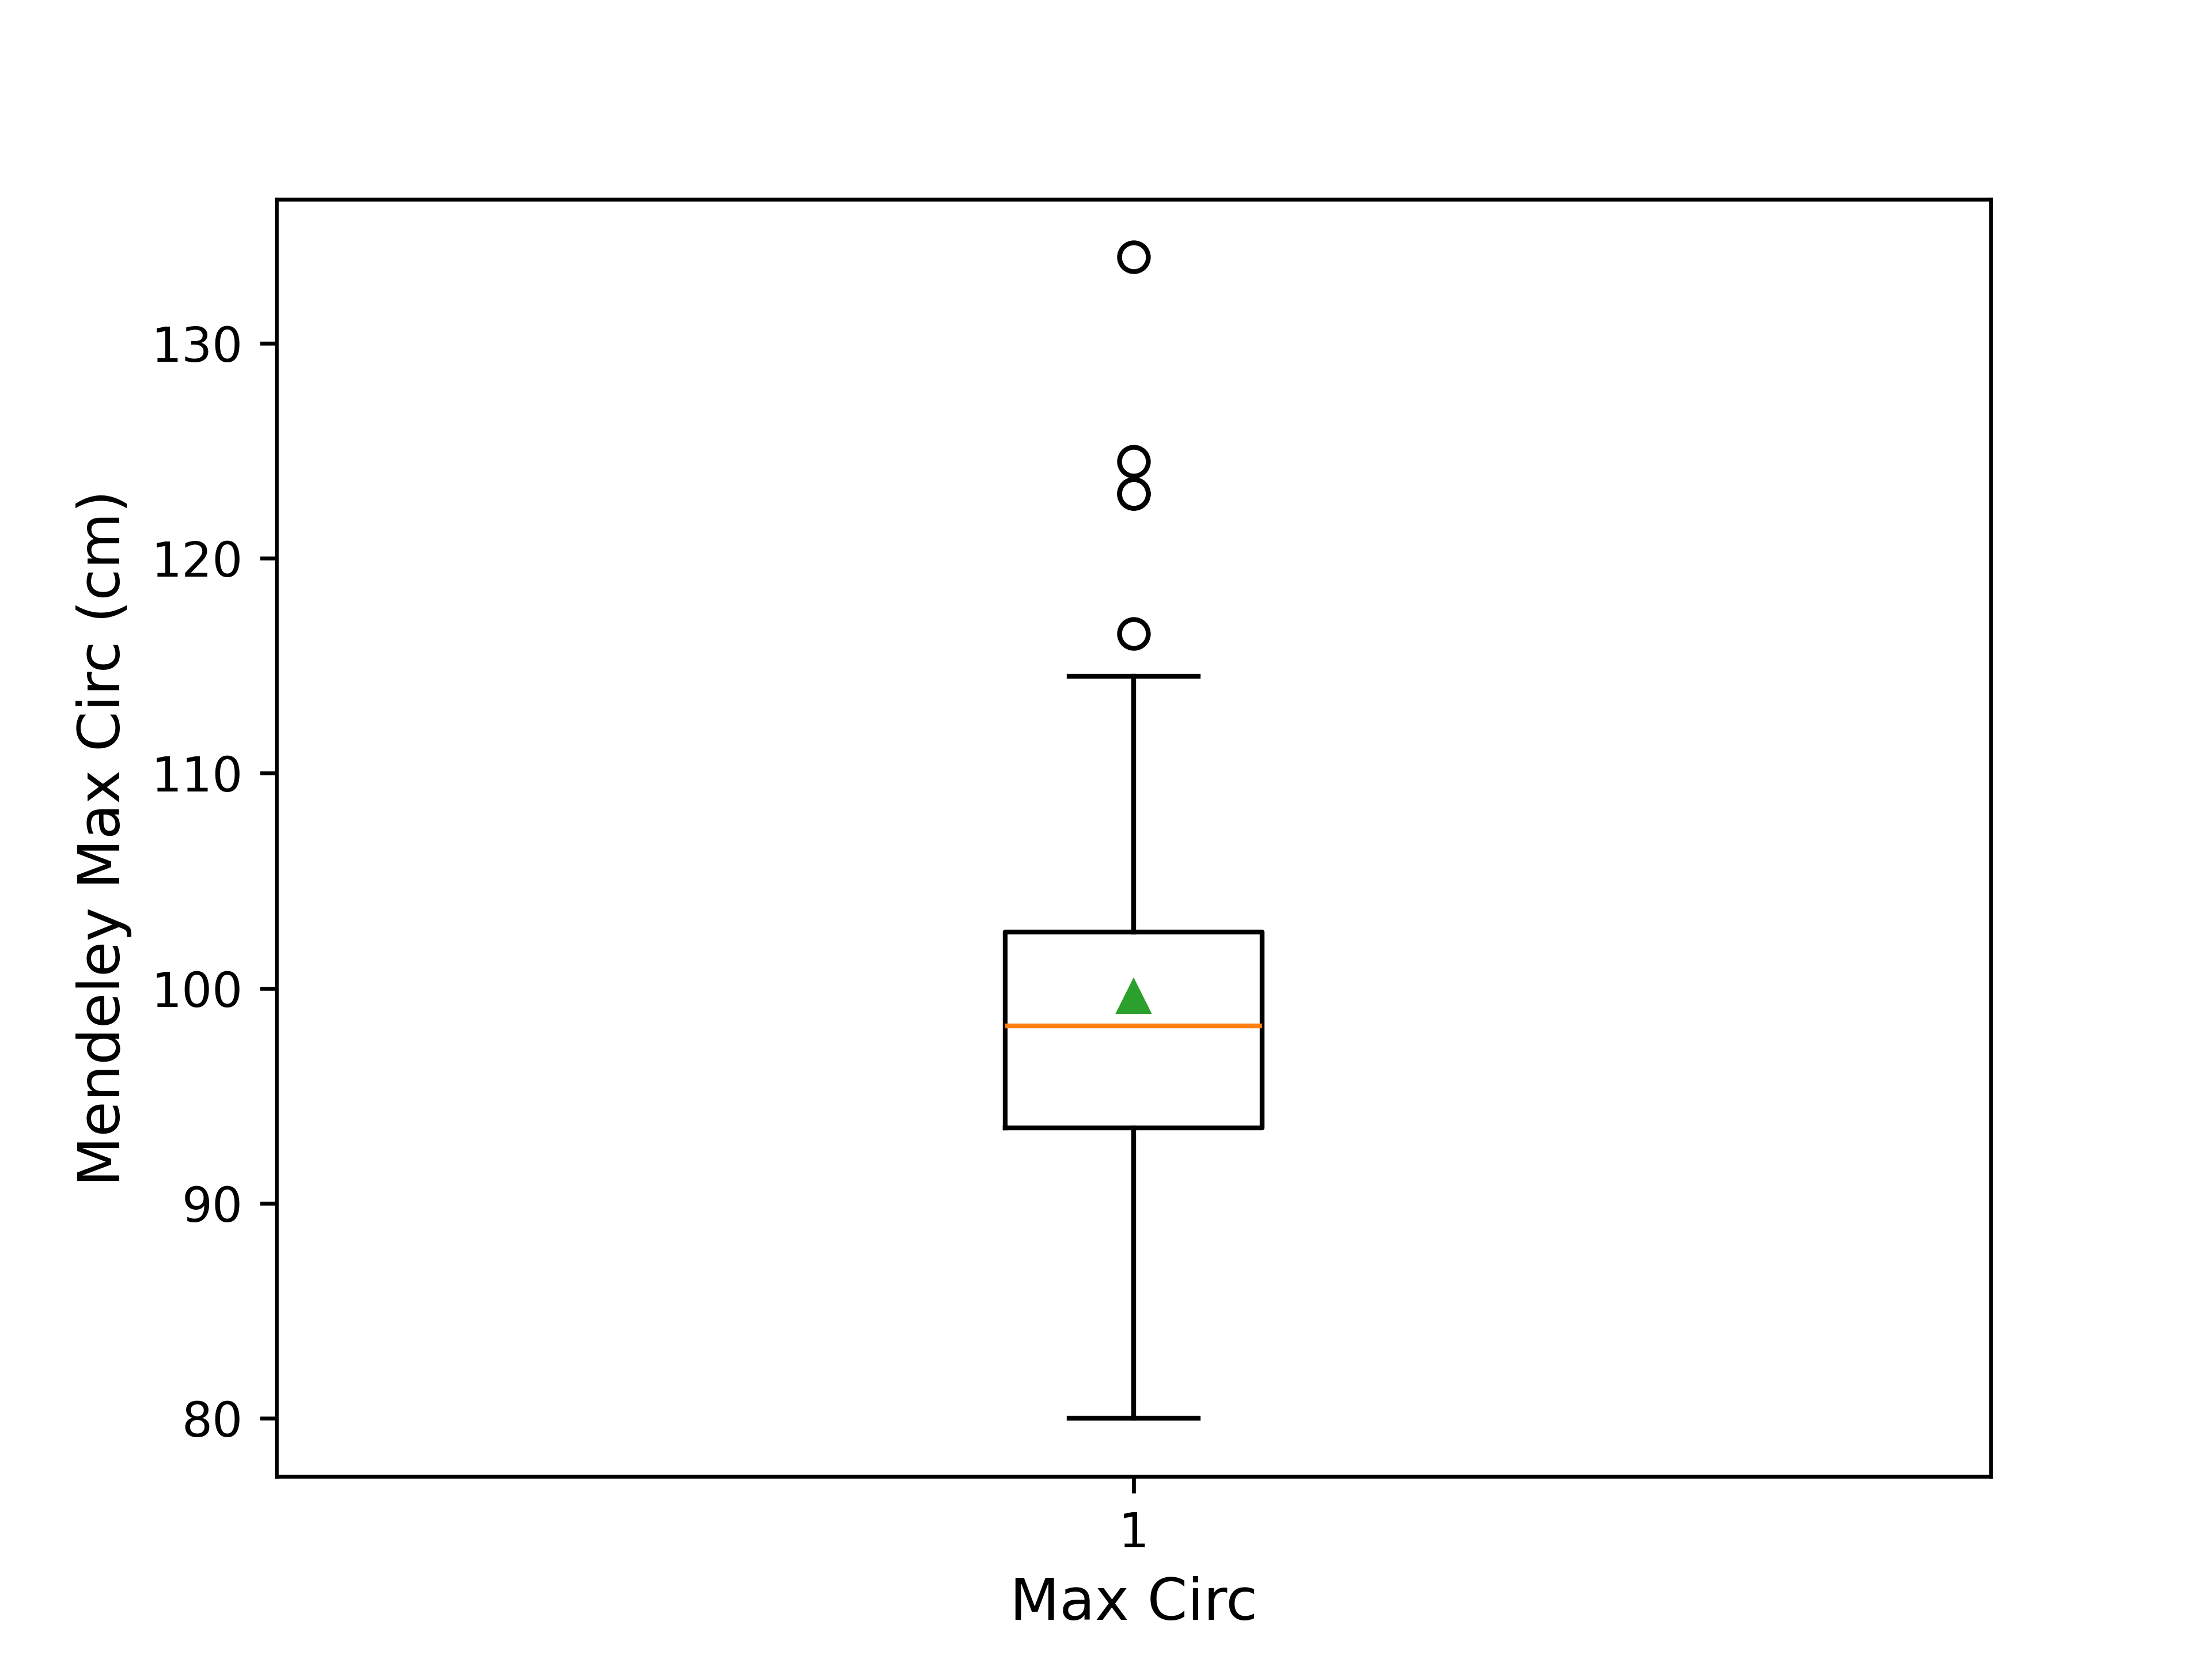
\includegraphics[width=\textwidth]{Images/Mendeley_max_circ_Boxplot.png}
        \caption{Boxplot}
    \end{subfigure}
    \caption{Distribution of max bodice circumference for 100 Scans Study}
\end{figure}

\subsubsection{Fabric Use}
Efficiency, bolt width, cut loss width, and cut loss area for 100 scans study comparing ideal bolt and hypothetical used bolt.
When using the ideal bolt width, the mean efficiency is 98\%, median efficiency is 98\%, and the standard deviation is 1\%. The mean ideal bolt width is 133 cm and median ideal bolt is 130 cm.
\begin{figure} [H] % opens the figure environment. the '[H]' forces the image to be Here
    \centering % puts the image in the horizontal centre of the page
    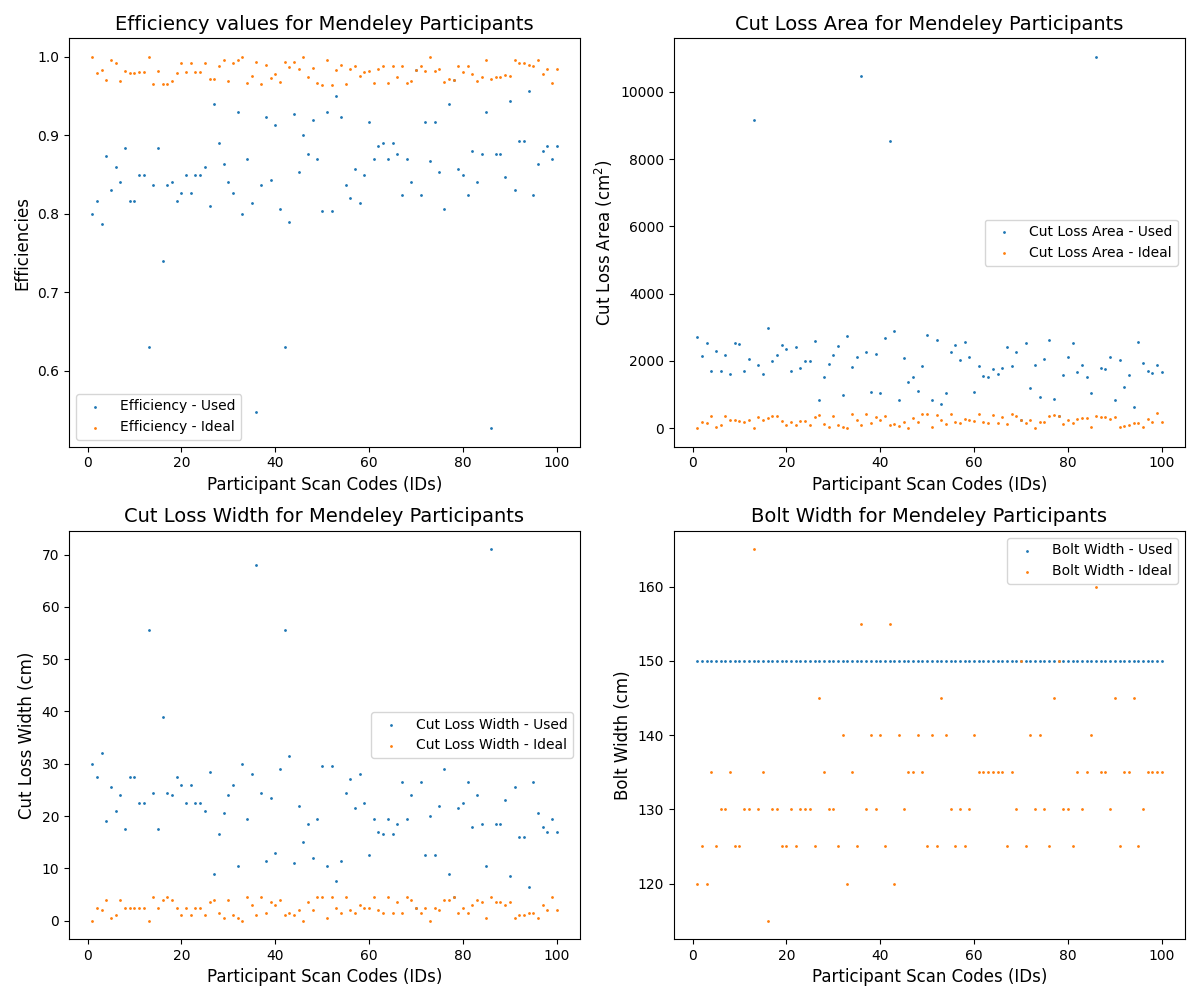
\includegraphics[width = \textwidth]{Images/Mendeley_Plot.png} %this tells latex what graphics to include. I put my images in an 'Images' folder to aid file management, hence the Images/ before the file name. the width bit before allows you to alter the width of the image. It is also possible to use scale as well as using equations with the textwidth to make it say half the text width.
    \caption{Used and Ideal Efficiency Metrics for 100 Scans Study}
\end{figure}

Cohort analysis
\begin{verbatim}
For bolt width 110
efficiency_used Mean: 0.8172272727272727
efficiency_used Median: 0.8363636363636363
efficiency_used Standard Deviation: 0.06112003837457149
cut_loss_area_used Mean: 2620.64
cut_loss_area_used Median: 2318.0
cut_loss_area_used Standard Deviation: 889.3173086137477

For bolt width 115
efficiency_used Mean: 0.7846956521739128
efficiency_used Median: 0.8
efficiency_used Standard Deviation: 0.060083369930081405
cut_loss_area_used Mean: 3233.865
cut_loss_area_used Median: 2922.75
cut_loss_area_used Standard Deviation: 937.4587907076235

For bolt width 120
efficiency_used Mean: 0.7622500000000001
efficiency_used Median: 0.7708333333333334
efficiency_used Standard Deviation: 0.07380252366958734
cut_loss_area_used Mean: 3737.44
cut_loss_area_used Median: 3556.875
cut_loss_area_used Standard Deviation: 1207.1684768084363

For bolt width 125
efficiency_used Mean: 0.78652
efficiency_used Median: 0.756
efficiency_used Standard Deviation: 0.12139279056023056
cut_loss_area_used Mean: 3526.84
cut_loss_area_used Median: 4025.0
cut_loss_area_used Standard Deviation: 2097.150328278829

For bolt width 130
efficiency_used Mean: 0.8370769230769229
efficiency_used Median: 0.9173076923076924
efficiency_used Standard Deviation: 0.13486956223169128
cut_loss_area_used Mean: 2771.99
cut_loss_area_used Median: 934.5
cut_loss_area_used Standard Deviation: 2542.7475641321535

For bolt width 135
efficiency_used Mean: 0.8791851851851853
efficiency_used Median: 0.9296296296296296
efficiency_used Standard Deviation: 0.12263318115152018
cut_loss_area_used Mean: 1997.815
cut_loss_area_used Median: 843.0
cut_loss_area_used Standard Deviation: 2501.28740817104

For bolt width 140
efficiency_used Mean: 0.888107142857143
efficiency_used Median: 0.9107142857142857
efficiency_used Standard Deviation: 0.09240419059098733
cut_loss_area_used Mean: 1716.44
cut_loss_area_used Median: 1131.0
cut_loss_area_used Standard Deviation: 2025.6374827199463

For bolt width 145
efficiency_used Mean: 0.8732758620689655
efficiency_used Median: 0.8810344827586207
efficiency_used Standard Deviation: 0.08091241723482498
cut_loss_area_used Mean: 1865.09
cut_loss_area_used Median: 1491.625
cut_loss_area_used Standard Deviation: 1849.1465333769522

For bolt width 150
efficiency_used Mean: 0.8519666666666669
efficiency_used Median: 0.855
efficiency_used Standard Deviation: 0.07106819104056172
cut_loss_area_used Mean: 2158.84
cut_loss_area_used Median: 1890.75
cut_loss_area_used Standard Deviation: 1679.2237014168184

For bolt width 155
efficiency_used Mean: 0.8329677419354837
efficiency_used Median: 0.8306451612903225
efficiency_used Standard Deviation: 0.06241344474812926
cut_loss_area_used Mean: 2418.415
cut_loss_area_used Median: 2333.625
cut_loss_area_used Standard Deviation: 1388.6237018267402

For bolt width 160
efficiency_used Mean: 0.8117187499999998
efficiency_used Median: 0.80625
efficiency_used Standard Deviation: 0.05407491728784705
cut_loss_area_used Mean: 2752.84
cut_loss_area_used Median: 2795.125
cut_loss_area_used Standard Deviation: 1076.7399033192744

For bolt width 165
efficiency_used Mean: 0.7913939393939395
efficiency_used Median: 0.7833333333333333
efficiency_used Standard Deviation: 0.05219994054086801
cut_loss_area_used Mean: 3089.515
cut_loss_area_used Median: 3250.125
cut_loss_area_used Standard Deviation: 782.1969140024779
\end{verbatim}

Best bolt for the cohort is 135/140 ??

Count of pattern orientation on starting fabric and possibility of embellishment potential for various bolt widths ranging from 110 to 160 cm.
\begin{figure} [H] % opens the figure environment. the '[H]' forces the image to be Here
    \centering % puts the image in the horizontal centre of the page
    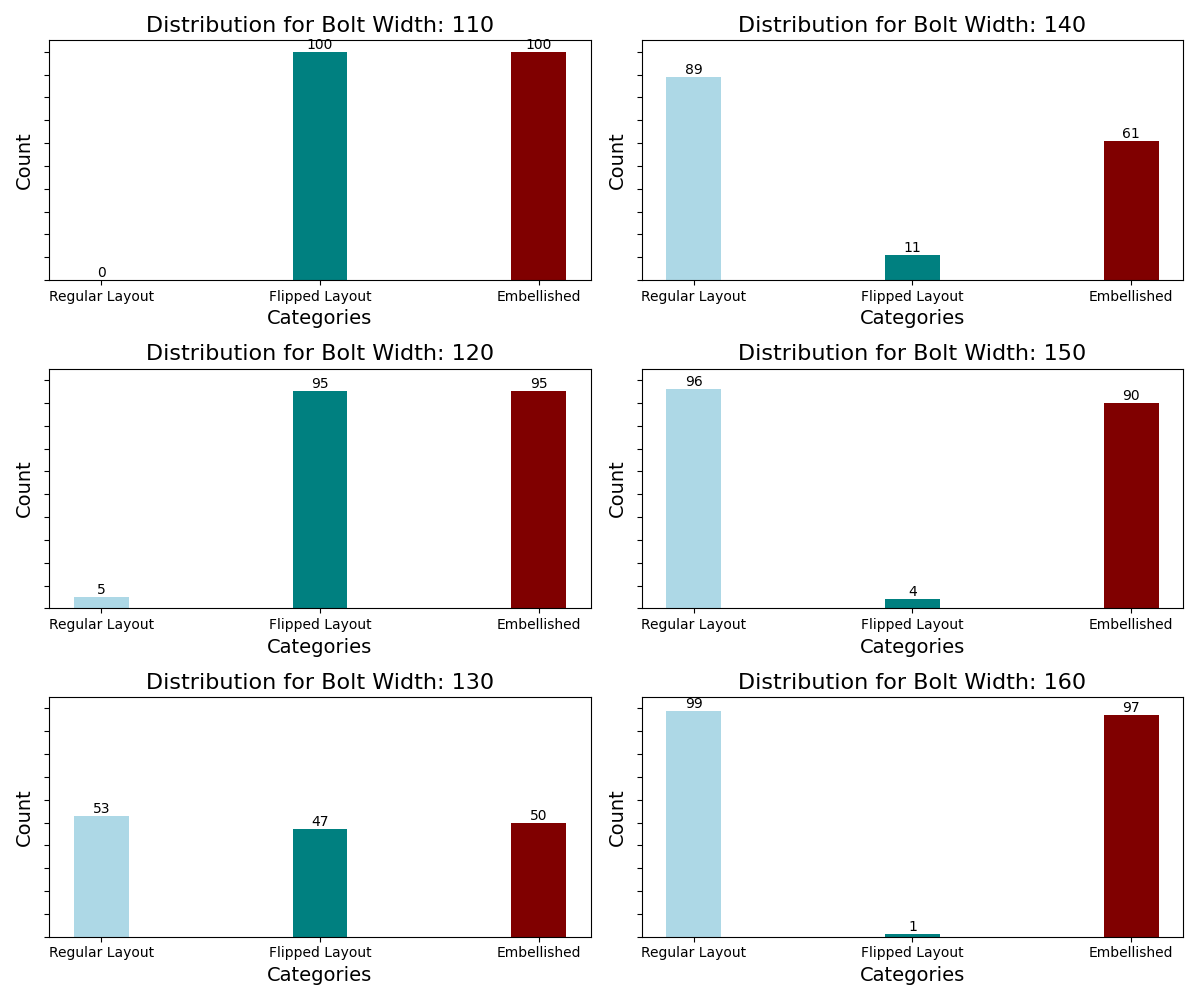
\includegraphics[width = \textwidth]{Images/Mendeley_Bar.png} %this tells latex what graphics to include. I put my images in an 'Images' folder to aid file management, hence the Images/ before the file name. the width bit before allows you to alter the width of the image. It is also possible to use scale as well as using equations with the textwidth to make it say half the text width.
    \caption{Layout and Embellishment Possibility for 100 Scans Study}
\end{figure}

ADD recoup of cut loss area due to embellishment